\chapter*{Preliminaries}
This protocol is a general review of the practicum Wireless Digital Communications Lab I, where two students work together at one PC as a group. The main task is to detect and receive the signal from  wireless channel under the UMTS structure. 

UMTS (Universal Mobile Telecommunications System) is a \nth{3} generation cellular mobile communication system and standardized by 3GPP (Third Generation Partnership Project). Several air interface (physical layer) specifications have been introduced:
\begin{itemize}
	\item UTRA FDD
	\item UTRA TDD
	\item CDMA 2000
\end{itemize}

\section{Signal Structure}
\subsection{Complex phase modulation: QPSK}
The Quadrature Phase-Shift Keying (QPSK) uses four points on the constellation diagram. After modulation each symbol contains 2 information bits. The mapping table is defined as follow:
\begin {table}[H]
\centering
\begin{tabular}{|c|c|}
	
	\hline
	Consecutive binary bit pattern & complex symbol \\    \hline
	00 & +j \\   \hline
	01 & +1 \\   \hline
	10 & -1 \\   \hline
	11 & -j \\   \hline

\end{tabular}
\caption {QPSK Mapping Table}
\end{table}

\subsection{Transmit pulse shape filter}
The transmit pulse-shaping filter is a root-raised cosine (RRC) with roll-off 0.22 in the frequency domain. The impulse response of the chip impulse filter $\text{RC}_0(t)$ is:
$$ \text{RC}_0(t) = \frac{\sin \left(\pi \frac{t}{T_C}(1-\alpha)\right) + 4\alpha \frac{t}{T_C} \cos \left( \pi \frac{t}{T_C}(1+\alpha) \right)}{\pi \frac{t}{T_C} \left( 1-\left( 4 \alpha \frac{t}{T_C} \right)^2 \right)} $$
Where the roll-off factor $\alpha = 0.22$ and the chip duration:
$T_C = \frac{1}{chiprate} \approx 0.26042 \mu s$

\subsection{CDMA Spreading}
Spreading codes are used for different users. These codes require the property of good auto- and cross-correlation function. Since the multiplication of two Hadamard matrix produces an identity matrix. We can make use of the columns of the matrix (based on Walsh sequences) as the Spreading code. The code-tree for generation of Orthogonal Variable Spreading Factor (OVSF) codes for channelization Operation is shown in Figure \ref{fig:pre:spreading}.

\begin{figure}
	\begin{center}
		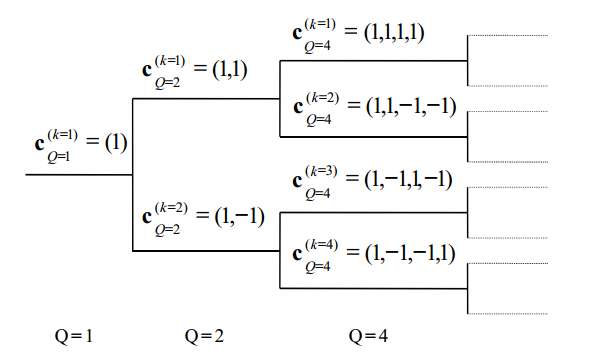
\includegraphics[scale=0.5]{pre/spreading.png}
		\caption{OVSF code tree \citealp{e1}}
		\label{fig:pre:spreading}
	\end{center}
\end{figure}

\subsection{Scrambling}
Since adjacent cells use the same carrier frequency, signal separation of different base stations is realized by particular scrambling sequences which are specific for adjacent cells. These scrambling sequences are complex valued and have a fixed length of 16 elements (\emph{aka.} chips). 16 consecutive chips of the spread data are element-wise multiplied by the given scrambling sequence, which is called Hadamard vector product.

\subsection{Burst Types}
\begin{table}[H]
\centering
\begin{tabular}{|c|c|}
	\hline
	Midamble Length & Use Case \\ \hline
	512 & uplink \& downlink: independent of the number of active users in one time slot \\ \hline
	256 & uplink: if the bursts within a time slot are allocated to less than four users\\ 
	& downlink: independent of number of the number of active users in one time slot\\
	\hline	
\end{tabular}
\end{table}

\subsection{Timeslot Structure}
A timeslot is composed of 3 parts: two data parts and the midamble part, which is shown in figure \ref{fig:pre:timeslot}.
\begin{figure}[H]
	\begin{center}
		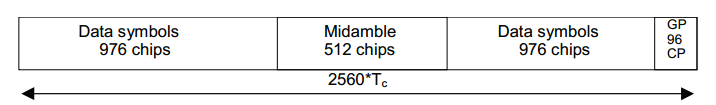
\includegraphics[scale=0.5]{pre/timeslot.png}
		\caption{Time slots \cite{e1}}
		\label{fig:pre:timeslot}
	\end{center}
\end{figure}

\subsection{Midamble sequences}
Midamble sequences are applied for channel estimation and synchronization. For the UTRA TDD midamble sequences, adjacent base stations use different midamble sequences. In downlink the mobile station can estimate their individual channel state information by receiving the midamble sequences from the BS, while in uplink, the BS will receive a superimposed version of the midambles from all the mobile stations, each of which is derived from a cyclic shift of a basic midamble.

\section{The SDR platform (Wireless Experimental System II)}
The SDR platform is used for remote controlled indoor transmission from one or two transmit antenna(s) to one or two receive antenna(s). The carrier frequency varies from 2000 to 2500 MHz. There are two base band signal bandwidth: 250M Hz (wideband mode) or 15.625 MHz (downsampled). The approximate transmit power is -6dBm (\SI{250}{\micro \watt}). The offline signal processing will be done with Matlab. The sampling frequency for UMTS and WLAN transmission experiments is 15.625 Msps (4 samples per UMTS-CDMA-chip).

Every group uses a SDR device connected to a host notebook via a PCIe interface. All working groups can use a remote control Matlab function, called "RemoteTransmission()" to have access to the SDR device.  This function requires a parameter with Matlab parameter structure "TransmissionParameter", which contains information like transmit power, the antenna attenuation for both transmitter and receiver, the name of existing transmit signals and bandwidth.

After running the RemoteTransmission() a Matlab data file will be generated, which involves the received signal samples, status information of the SDR system during the transmission, as well as a string variable whose name is the transmit signal. The received signal samples comprise in-phase and quadrature component signal samples, cell-array with messages about the transmission procedure, Group ID, bandwidth, transmission parameter structure and system parameters that were active during the transmission.  
\section{Organization of this Protocol}
Our first experiment is dealing with a single transmit signal of a mobile station, which is transmitted to a base station over DPCH (uplink). There will be no multipath propagation effects and hence a simple match filter receiver is sufficient to receive and detect the signal.